\documentclass{extbook}[14pt]
\usepackage{multicol, enumerate, enumitem, hyperref, color, soul, setspace, parskip, fancyhdr, amssymb, amsthm, amsmath, bbm, latexsym, units, mathtools}
\everymath{\displaystyle}
\usepackage[headsep=0.5cm,headheight=0cm, left=1 in,right= 1 in,top= 1 in,bottom= 1 in]{geometry}
\pagestyle{fancy}
\lhead{}
\chead{Answer Key for Module\,6\,-\,Polynomial\,Functions Version A}
\rhead{}
\lfoot{Summer\,C\,2020}
\cfoot{}
\rfoot{}
\begin{document}
\textbf{This key should allow you to understand why you choose the option you did (beyond just getting a question right or wrong). \href{https://xronos.clas.ufl.edu/mac1105spring2020/courseDescriptionAndMisc/Exams/LearningFromResults}{More instructions on how to use this key can be found here}.}

\textbf{If you have a suggestion to make the keys better, \href{https://forms.gle/CZkbZmPbC9XALEE88}{please fill out the short survey here}.}

\textit{Note: This key is auto-generated and may contain issues and/or errors. The keys are reviewed after each exam to ensure grading is done accurately. If there are issues (like duplicate options), they are noted in the offline gradebook. The keys are a work-in-progress to give students as many resources to improve as possible.}

\rule{\textwidth}{0.4pt}

26. Construct the lowest-degree polynomial given the zeros below. Then, choose the intervals that contain the coefficients of the polynomial in the form $ax^3+bx^2+cx+d$.
\[ \frac{4}{5}, \frac{-7}{4}, \text{ and } \frac{5}{3} \] 
The solution is $ 60x^{3} -43 x^{2} -179 x + 140 $ 

\begin{enumerate}[label=\Alph*.] 
\item $ a \in [57, 68], b \in [52, 55], c \in [-173, -166], \text{ and } d \in [-143, -138] $ 

 $60x^{3} +53 x^{2} -171 x -140$, which corresponds to multiplying out $(5x + 5)(4x -4)(3x -3)$. 
\item $ a \in [57, 68], b \in [42, 47], c \in [-186, -177], \text{ and } d \in [-143, -138] $ 

 $60x^{3} +43 x^{2} -179 x -140$, which corresponds to multiplying out $(5x + 4)(4x -7)(3x + 5)$. 
\item $ a \in [57, 68], b \in [-48, -38], c \in [-186, -177], \text{ and } d \in [137, 145] $ 

 * $60x^{3} -43 x^{2} -179 x + 140$, which is the correct option. 
\item $ a \in [57, 68], b \in [-48, -38], c \in [-186, -177], \text{ and } d \in [-143, -138] $ 

 $60x^{3} -43 x^{2} -179 x -140$, which corresponds to multiplying everything correctly except the constant term. 
\item $ a \in [57, 68], b \in [-165, -155], c \in [8, 12], \text{ and } d \in [137, 145] $ 

 $60x^{3} -157 x^{2} +11 x + 140$, which corresponds to multiplying out $(5x + 5)(4x + 4)(3x -3)$. 
\end{enumerate} 
 
General Comments: To construct the lowest-degree polynomial, you want to multiply out $(5x -4)(4x + 7)(3x -5)$

-----------------------------------------------

27. Describe the zero behavior of the zero $x = 5$ of the polynomial below.
\[ f(x) = 2(x + 6)^{11}(x - 6)^{8}(x + 5)^{9}(x - 5)^{8} \] 

 
 The solution is  
 \begin{center} 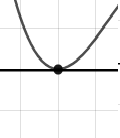
\includegraphics[width=0.3\textwidth]{../Figures/polyZeroBehaviorCA.png} \end{center}\begin{tabular}{|c|c|} 
\hline 
 & \tabularnewline 
 \textbf{A.} 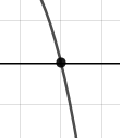
\includegraphics[width=0.3\textwidth]{../Figures/polyZeroBehaviorAA.png} & \textbf{B.} 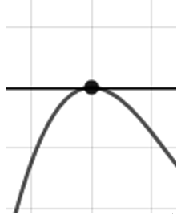
\includegraphics[width=0.3\textwidth]{../Figures/polyZeroBehaviorBA.png} \tabularnewline 
\hline 
 & \tabularnewline 
 \textbf{C.} 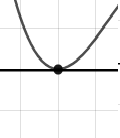
\includegraphics[width=0.3\textwidth]{../Figures/polyZeroBehaviorCA.png} & \textbf{D.} 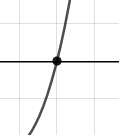
\includegraphics[width=0.3\textwidth]{../Figures/polyZeroBehaviorDA.png} \tabularnewline 
\hline 
 E. None of the figures above. & \tabularnewline 
\hline 
 \end{tabular} 
 
\begin{enumerate}[label=\Alph*.] 
\item   
\item   
\item   
\item   
\end{enumerate} 
 
\textbf{General Comments:} You will need to sketch the entire graph, then zoom in on the zero the question asks about.

-----------------------------------------------

28. Which of the following equations \textit{could} be of the graph presented below?
\begin{center} 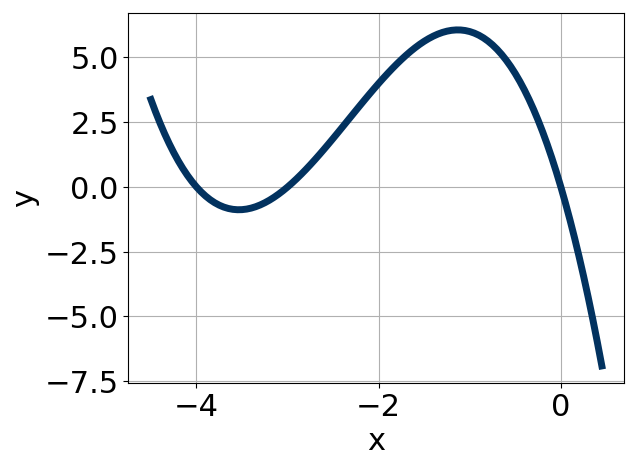
\includegraphics[width=0.3\textwidth]{../Figures/polyGraphToFunctionA.png} \end{center} 

The solution is $ 19x^{8} (x - 1)^{7} (x + 4)^{5} $ 

\begin{enumerate}[label=\Alph*.] 
\item $ 19x^{8} (x - 1)^{7} (x + 4)^{5} $ 

 * This is the correct option. 
\item $ -18x^{10} (x - 1)^{9} (x + 4)^{11} $ 

 This corresponds to the leading coefficient being the opposite value than it should be. 
\item $ 19x^{10} (x - 1)^{4} (x + 4)^{7} $ 

 The factor $(x - 1)$ should have an odd power. 
\item $ -15x^{6} (x - 1)^{9} (x + 4)^{4} $ 

 The factor $(x + 4)$ should have an odd power and the leading coefficient should be the opposite sign. 
\item $ 17x^{7} (x - 1)^{6} (x + 4)^{7} $ 

 The factor $0$ should have an even power and the factor $1$ should have an odd power. 
\end{enumerate} 
 
General Comments: Draw the x-axis to determine which zeros are touching (and so have even multiplicity) or cross (and have odd multiplicity).

-----------------------------------------------

29. Describe the end behavior of the polynomial below.
\[ f(x) = -3(x - 9)^{2}(x + 9)^{3}(x + 2)^{4}(x - 2)^{6} \] 

 
 The solution is  
 \begin{center} 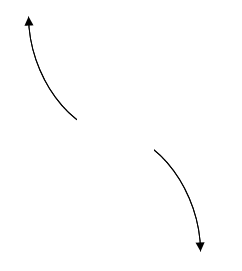
\includegraphics[width=0.3\textwidth]{../Figures/polyEndBehaviorAA.png} \end{center}\begin{tabular}{|c|c|} 
\hline 
 & \tabularnewline 
 \textbf{A.} 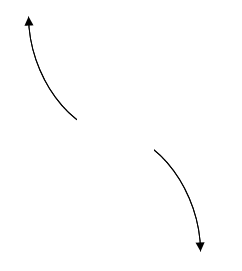
\includegraphics[width=0.3\textwidth]{../Figures/polyEndBehaviorAA.png} & \textbf{B.} 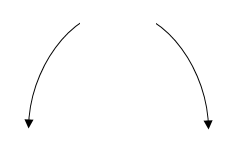
\includegraphics[width=0.3\textwidth]{../Figures/polyEndBehaviorBA.png} \tabularnewline 
\hline 
 & \tabularnewline 
 \textbf{C.} 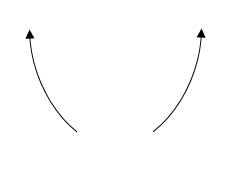
\includegraphics[width=0.3\textwidth]{../Figures/polyEndBehaviorCA.png} & \textbf{D.} 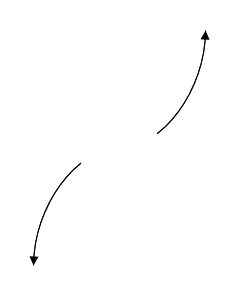
\includegraphics[width=0.3\textwidth]{../Figures/polyEndBehaviorDA.png} \tabularnewline 
\hline 
 E. None of the figures above. & \tabularnewline 
\hline 
 \end{tabular} 
 
\begin{enumerate}[label=\Alph*.] 
\item The function is above the $x$-axis, then passes through.  
\item The function is below the $x$-axis, then touches.  
\item The function is above the $x$-axis, then touches.  
\item The function is below the $x$-axis, then passes through.  
\end{enumerate} 
 
\textbf{General Comments:} Remember that end behavior is determined by the leading coefficient AND whether the \textbf{sum} of the multiplicities is positive or negative.

-----------------------------------------------

30. Construct the lowest-degree polynomial given the zeros below. Then, choose the intervals that contain the coefficients of the polynomial in the form $x^3+bx^2+cx+d$.
\[ 3 + 4i \text{ and } -4 \] 
The solution is $ x^{3} -2 x^{2} +x + 100 $ 

\begin{enumerate}[label=\Alph*.] 
\item $ b \in [0.9, 1.29], c \in [0.57, 2.03], \text{ and } d \in [-15, -9] $ 

 $x^{3} + x^{2} +x -12$, which corresponds to multiplying out $(x -3)(x + 4)$. 
\item $ b \in [0.9, 1.29], c \in [-0.81, 0.51], \text{ and } d \in [-23, -14] $ 

 $x^{3} + x^{2} -16$, which corresponds to multiplying out $(x -4)(x + 4)$. 
\item $ b \in [-2.11, -1.02], c \in [0.57, 2.03], \text{ and } d \in [98, 102] $ 

 * $x^{3} -2 x^{2} +x + 100$, which is the correct option. 
\item $ b \in [1.03, 2.65], c \in [0.57, 2.03], \text{ and } d \in [-101, -98] $ 

 $x^{3} +2 x^{2} +x -100$, which corresponds to multiplying out $(x-(3 + 4i))(x-(3 - 4i))(x -4)$. 
\item $ \text{None of the above.} $ 

 This corresponds to making an unanticipated error or not understanding how to use nonreal complex numbers to create the lowest-degree polynomial. If you chose this and are not sure what you did wrong, please contact the coordinator for help. 
\end{enumerate} 
 
General Comments: Remember that the conjugate of $a+bi$ is $a-bi$. Since these zeros always come in pairs, we need to multiply out $(x-(3 + 4i))(x-(3 - 4i))(x-(-4))$.

-----------------------------------------------


\end{document}

